\chapter{Notes on the Koopman Inference Algorithm}



\section{Full Derivation}
	\label{app:fullNgkDerivation}

	In this appendix we cover the full derivation of the Koopman inference algorithm, starting with the formulation of the expected log-likelihood, going over the M-step and finally to the E-step with the regular, non-square-root, filter/smoother equations.

	Our model is given as
	This model can also be written as a set of both linear and nonlinear equations:
	\begin{align*}
		p(\vec{s}_t \given \vec{s}_{t - 1}) &\sim \normal(\mat{A} \vec{s}_{t - 1}, \mat{Q}) \\
		p(\vec{y}_t \given \vec{s}_t)       &\sim \normal\big(\vec{g}(\vec{s}_t), \mat{R}\big)
	\end{align*}
	with diagonal noise covariances \(\mat{Q}\) and \(\mat{R}\).

	\paragraph{M-Step}
		For a single observation sequence, the log-likelihood \( \log p\Big(\vec{s}_{1:T}^{(n)}, \vec{y}_{1:T}^{(n)}\Big) \) is given as
		\begin{align*}
			\log p\Big(\vec{s}_{1:T}^{(n)}, \vec{y}_{1:T}^{(n)}\Big)
				&= \log \Bigg(\! p\Big(\vec{s}_1^{(n)}\Big) \prod_{t = 2}^{T} p\Big(\vec{s}_t^{(n)} \given \vec{s}_{t - 1}^{(n)}\Big) \prod_{t = 1}^{T} p\Big(\vec{y}_t^{(n)} \given \vec{s}_t^{(n)}\Big) \!\Bigg) \\
				&= \log p\Big(\vec{s}_1^{(n)}\Big) + \sum_{t = 2}^{T} \log p\Big(\vec{s}_t^{(n)} \given \vec{s}_{t - 1}^{(n)}\Big) + \sum_{t = 1}^{T} \log p\Big(\vec{y}_t^{(n)} \given \vec{s}_t^{(n)}\Big) \\
				&= \logGaussianMulti{\vec{s}_1^{(n)}}{\vec{m}_0}{\mat{V}_0}{k} \\
				&\qquad\qquad + \sum_{t = 2}^{T} \logGaussianMulti{\vec{s}_t^{(n)}}{\mat{A} \vec{s}_{t - 1}^{(n)}}{\mat{Q}}{k} \\
				&\qquad\qquad + \sum_{t = 1}^{T} \logGaussianMulti{\vec{y}_t^{(n)}}{\vec{g}_t^{(n)}}{\mat{R}}{p} \\
				&= -\frac{T(k + p)}{2} \log(2\pi) - \frac{1}{2} \log \lvert \mat{V}_0 \rvert - \frac{T - 1}{2} \log \lvert \mat{Q} \rvert - \frac{T}{2} \log \lvert \mat{R} \rvert \\
				&\qquad\qquad -\frac{1}{2} \Big( \vec{s}_1^{(n)} - \vec{m}_0 \Big)^T \mat{V}_0^{-1} \Big( \vec{s}_1^{(n)} - \vec{m}_0 \Big) \\
				&\qquad\qquad -\frac{1}{2} \sum_{t = 2}^{T} \Big( \vec{s}_t^{(n)} - \mat{A} \vec{s}_{t - 1}^{(n)} \Big)^T \mat{Q}^{-1} \Big( \vec{s}_t^{(n)} - \mat{A} \vec{s}_{t - 1}^{(n)} \Big) \\
				&\qquad\qquad -\frac{1}{2} \sum_{t = 1}^{T} \Big( \vec{y}_t^{(n)} - \vec{g}_t^{(n)} \Big)^T \mat{R}^{-1} \Big( \vec{y}_t^{(n)} - \vec{g}_t^{(n)} \Big)
		\end{align*}
		as the system behaves Markovian and \( \vec{m}_0 \) and \( \mat{V}_0 \) are the initial state mean and covariance. We assume the observation sequences to be \ac{iid}, we can formulate the joint complete log-likelihood \( \log p(\vec{s}_{1:T}, \vec{y}_{1:T}) \) as the sum of all subsequent log-likelihoods:
		\begin{align*}
			\log p(\vec{s}_{1:T}, \vec{y}_{1:T})
				&= \log \prod_{n = 1}^{N} p\Big(\vec{s}_{1:T}^{(n)}, \vec{y}_{1:T}^{(n)}\Big) = \sum_{n = 1}^{N} \log p\Big(\vec{s}_{1:T}^{(n)}, \vec{y}_{1:T}^{(n)}\Big) \\
				&= -\frac{NT(k + p)}{2} \log(2\pi) - \frac{N}{2} \log \lvert \mat{V}_0 \rvert - \frac{N(T - 1)}{2} \log \lvert \mat{Q} \rvert - \frac{NT}{2} \log \lvert \mat{R} \rvert \\
				&\qquad\qquad -\frac{1}{2} \sum_{n = 1}^{N} \Big( \vec{s}_1^{(n)} - \vec{m}_0 \Big)^T \mat{V}_0^{-1} \Big( \vec{s}_1^{(n)} - \vec{m}_0 \Big) \\
				&\qquad\qquad -\frac{1}{2} \sum_{n = 1}^{N} \sum_{t = 2}^{T} \Big( \vec{s}_t^{(n)} - \mat{A} \vec{s}_{t - 1}^{(n)} \Big)^T \mat{Q}^{-1} \Big( \vec{s}_t^{(n)} - \mat{A} \vec{s}_{t - 1}^{(n)} \Big) \\
				&\qquad\qquad -\frac{1}{2} \sum_{n = 1}^{N} \sum_{t = 1}^{T} \Big( \vec{y}_t^{(n)} - \vec{g}_t^{(n)} \Big)^T \mat{R}^{-1} \Big( \vec{y}_t^{(n)} - \vec{g}_t^{(n)} \Big)
		\end{align*}
		To derive the M-step formulas, we need to maximize the \emph{expected} log-likelihood. Therefore, we will now derive the expected log-likelihood
		\begin{equation*}
			Q = \E\big[ p(\vec{s}_{1:T}, \vec{y}_{1:T}) \given \vec{y}_{1:T} \big]
		\end{equation*}
		This quantity depends on five expectations \( \hat{\vec{s}}_{t \subgiven t_0}^{(n)} \), \( \mat{P}_{t \subgiven t_0}^{(n)} \), \( \mat{P}_{t, t - 1 \subgiven t_0}^{(n)} \), \( \hat{\vec{g}}_t^{(n)} \) and \( \mat{G}_{t}^{(n)} \) as defined in equations~\eqref{eq:stateSmoothed} through~\eqref{eq:expectedMeasurementMat} in~\autoref{sec:ngkDerivation}. For brevity, let
		\begin{align*}
			q_1 &\coloneqq -\frac{NT(k + p)}{2} \log(2\pi) - \frac{N}{2} \log \lvert \mat{V}_0 \rvert - \frac{N(T - 1)}{2} \log \lvert \mat{Q} \rvert - \frac{NT}{2} \log \lvert \mat{R} \rvert \\
			q_2 &\coloneqq -\frac{1}{2} \sum_{n = 1}^{N} \Big( \vec{s}_1^{(n)} - \vec{m}_0 \Big)^T \mat{V}_0^{-1} \Big( \vec{s}_1^{(n)} - \vec{m}_0 \Big) \\
			q_3 &\coloneqq -\frac{1}{2} \sum_{n = 1}^{N} \sum_{t = 2}^{T} \Big( \vec{s}_t^{(n)} - \mat{A} \vec{s}_{t - 1}^{(n)} \Big)^T \mat{Q}^{-1} \Big( \vec{s}_t^{(n)} - \mat{A} \vec{s}_{t - 1}^{(n)} \Big) \\
			q_4 &\coloneqq -\frac{1}{2} \sum_{n = 1}^{N} \sum_{t = 1}^{T} \Big( \vec{y}_t^{(n)} - \vec{g}_t^{(n)} \Big)^T \mat{R}^{-1} \Big( \vec{y}_t^{(n)} - \vec{g}_t^{(n)} \Big)
		\end{align*}
		such that \( \log p(\vec{s}_{1:T}, \vec{y}_{1:T}) = q_1 + q_2 + q_3 + q_4 \) and, with \(Q_1\), \(Q_2\), \(Q_3\) and \(Q_4\) being the corresponding expectations, \( Q = Q_1 + Q_2 + Q_3 + Q_4 \).

		We will now evaluate the respective expectations.
		\begin{itemize}
			\item Compute \(Q_1\):
		\end{itemize}
		\begin{equation*}
			Q_1 = \E[q_1 \given \vec{y}_{1:T}] = -\frac{NT(k + p)}{2} \ln(2\pi) - \frac{N}{2} \ln \lvert \mat{V}_0 \rvert - \frac{N(T - 1)}{2} \ln \lvert \mat{Q} \rvert - \frac{NT}{2} \ln \lvert \mat{R} \rvert
		\end{equation*}
		\pagebreak

		\begin{itemize}
			\item Compute \(Q_2\):
		\end{itemize}
		\begin{align*}
			Q_2
				&= \E[q_2 \given \vec{y}_{1:T}] \\
				&= \E\Bigg[\! -\frac{1}{2} \sum_{n = 1}^{N} \Big( \vec{s}_1^{(n)} - \vec{m}_0 \Big)^T \mat{V}_0^{-1} \Big( \vec{s}_1^{(n)} - \vec{m}_0 \Big) \Bigggiven \vec{y}_{1:T} \Bigg] \\
				&= -\frac{1}{2} \sum_{n = 1}^{N} \E\Bigg[ \Big( \vec{s}_1^{(n)} - \vec{m}_0 \Big)^T \mat{V}_0^{-1} \Big( \vec{s}_1^{(n)} - \vec{m}_0 \Big) \Bigggiven \vec{y}_{1:T} \Bigg] \\
				&= -\frac{1}{2} \sum_{n = 1}^{N} \E\Bigg[ \tr\!\bigg(\!\Big( \vec{s}_1^{(n)} - \vec{m}_0 \Big)^T \mat{V}_0^{-1} \Big( \vec{s}_1^{(n)} - \vec{m}_0 \Big)\!\bigg) \Bigggiven \vec{y}_{1:T} \Bigg] \\
				&= -\frac{1}{2} \sum_{n = 1}^{N} \E\Bigg[ \tr\!\bigg(\!\Big( \vec{s}_1^{(n)} - \vec{m}_0 \Big) \Big( \vec{s}_1^{(n)} - \vec{m}_0 \Big)^T \mat{V}_0^{-1} \!\bigg) \Bigggiven \vec{y}_{1:T} \Bigg] \\
				&= -\frac{1}{2} \sum_{n = 1}^{N} \E\Bigg[ \tr\!\bigg(\!\Big( \vec{s}_1^{(n)} - \vec{m}_0 \Big) \Big( \vec{s}_1^{(n), T} - \vec{m}_0^T \Big) \mat{V}_0^{-1} \!\bigg) \Bigggiven \vec{y}_{1:T} \Bigg] \\
				&= -\frac{1}{2} \sum_{n = 1}^{N} \E\Bigg[ \tr\!\bigg(\! \Big( \vec{s}_1^{(n)} \vec{s}_1^{(n), T} - \vec{s}_1^{(n)} \vec{m}_0^T - \vec{m} \vec{s}_1^{(n), T} + \vec{m}_0 \vec{m}_0^T \Big) \mat{V}_0^{-1} \!\bigg) \Bigggiven \vec{y}_{1:T} \Bigg] \\
				&= -\frac{1}{2} \sum_{n = 1}^{N} \tr\!\Big( \mat{P}_1^{(n)} \mat{V}_0^{-1} - \hat{\vec{s}}_1^{(n)} \vec{m}_0^T \mat{V}_0^{-1} - \vec{m} \hat{\vec{s}}_1^{(n), T} \mat{V}_0^{-1} + \vec{m}_0 \vec{m}_0^T \mat{V}_0^{-1} \Big) \\
				&= -\frac{1}{2} \sum_{n = 1}^{N} \tr\!\Big( \mat{P}_1^{(n)} \mat{V}_0^{-1} \Big) - \tr\!\Big( \hat{\vec{s}}_1^{(n)} \vec{m}_0^T \mat{V}_0^{-1} \Big) - \tr\!\Big( \vec{m}_0 \hat{\vec{s}}_1^{(n), T} \mat{V}_0^{-1} \Big) + \tr\!\Big(\vec{m}_0 \vec{m}_0^T \mat{V}_0^{-1} \Big) \\
				&=  -\frac{N}{2} \tr\!\Big( \mat{P}_1 \mat{V}_0^{-1} \Big) + \frac{N}{2} \tr\!\Big( \hat{\vec{s}}_1 \vec{m}_0^T \mat{V}_0^{-1} \Big) + \frac{N}{2} \tr\!\Big( \vec{m}_0 \hat{\vec{s}}_1^T \mat{V}_0^{-1} \Big) - \frac{N}{2} \tr\!\Big(\vec{m}_0 \vec{m}_0^T \mat{V}_0^{-1} \Big)
		\end{align*}
		\vfill
		\pagebreak

		\begin{itemize}
			\item Compute \(Q_3\):
		\end{itemize}
		\begin{align*}
			Q_3
				&= \E[q_3 \given \vec{y}_{1:T}] \\
				&= \E\Bigg[\! -\frac{1}{2} \sum_{n = 1}^{N} \sum_{t = 2}^{T} \Big( \vec{s}_t^{(n)} - \mat{A} \vec{s}_{t - 1}^{(n)} \Big)^T \mat{Q}^{-1} \Big( \vec{s}_t^{(n)} - \mat{A} \vec{s}_{t - 1}^{(n)} \Big) \Bigggiven \vec{y}_{1:T} \Bigg] \\
				&= -\frac{1}{2} \sum_{n = 1}^{N} \sum_{t = 2}^{T} \E\Bigg[ \Big( \vec{s}_t^{(n)} - \mat{A} \vec{s}_{t - 1}^{(n)} \Big)^T \mat{Q}^{-1} \Big( \vec{s}_t^{(n)} - \mat{A} \vec{s}_{t - 1}^{(n)} \Big) \Bigggiven \vec{y}_{1:T} \Bigg] \\
				&= -\frac{1}{2} \sum_{n = 1}^{N} \sum_{t = 2}^{T} \E\Bigg[ \tr\!\bigg(\!\Big( \vec{s}_t^{(n)} - \mat{A} \vec{s}_{t - 1}^{(n)} \Big)^T \mat{Q}^{-1} \Big( \vec{s}_t^{(n)} - \mat{A} \vec{s}_{t - 1}^{(n)} \Big)\!\bigg) \Bigggiven \vec{y}_{1:T} \Bigg] \\
				&= -\frac{1}{2} \sum_{n = 1}^{N} \sum_{t = 2}^{T} \E\Bigg[ \tr\!\bigg(\!\Big( \vec{s}_t^{(n)} - \mat{A} \vec{s}_{t - 1}^{(n)} \Big) \Big( \vec{s}_t^{(n)} - \mat{A} \vec{s}_{t - 1}^{(n)} \Big)^T \mat{Q}^{-1} \!\bigg) \Bigggiven \vec{y}_{1:T} \Bigg] \\
				&= -\frac{1}{2} \sum_{n = 1}^{N} \sum_{t = 2}^{T} \E\Bigg[ \tr\!\bigg(\!\Big( \vec{s}_t^{(n)} - \mat{A} \vec{s}_{t - 1}^{(n)} \Big) \Big(\vec{s}_t^{(n), T} - \vec{s}_{t - 1}^{(n), T} \mat{A}^T \Big) \mat{Q}^{-1} \!\bigg) \Bigggiven \vec{y}_{1:T} \Bigg] \\
				&= -\frac{1}{2} \sum_{n = 1}^{N} \sum_{t = 2}^{T} \E\Bigg[ \tr\!\bigg(\!\Big( \vec{s}_t^{(n)} \vec{s}_t^{(n), T} - \vec{s}_t^{(n)} \vec{s}_{t - 1}^{(n), T} \mat{A}^T - \mat{A} \vec{s}_{t - 1}^{(n)} \vec{s}_t^{(n), T} - \mat{A} \vec{s}_{t - 1}^{(n)} \vec{s}_{t - 1}^{(n), T} \mat{A}^T \Big) \mat{Q}^{-1} \!\bigg) \Bigggiven \vec{y}_{1:T} \Bigg] \\
				&= -\frac{1}{2} \sum_{n = 1}^{N} \sum_{t = 2}^{T} \tr\!\Big( \mat{P}_t^{(n)} \mat{Q}^{-1} - \mat{P}_{t, t - 1}^{(n)} \mat{A}^T \mat{Q}^{-1} - \mat{A} \underbrace{\mat{P}_{t - 1, t}^{(n)}}_{=\, \mat{P}_{t, t - 1}^{(n)}} \mat{Q}^{-1} - \mat{A} \mat{P}_{t - 1}^{(n)} \mat{A}^T \mat{Q}^{-1} \Big) \\
				&= -\frac{1}{2} \sum_{n = 1}^{N} \sum_{t = 2}^{T} \tr\!\Big( \mat{P}_t^{(n)} \mat{Q}^{-1} \Big) - \tr\!\Big( \mat{P}_{t, t - 1}^{(n)} \mat{A}^T \mat{Q}^{-1} \Big) - \tr\!\Big( \mat{A} \mat{P}_{t, t - 1}^{(n)} \mat{Q}^{-1} \Big) - \tr\!\Big( \mat{A} \mat{P}_{t - 1}^{(n)} \mat{A}^T \mat{Q}^{-1} \Big) \\
				&= -\frac{N}{2} \sum_{t = 2}^{T} \tr\!\Big( \mat{P}_t \mat{Q}^{-1} \Big) - \tr\!\Big( \mat{P}_{t, t - 1} \mat{A}^T \mat{Q}^{-1} \Big) - \tr\!\Big( \mat{A} \mat{P}_{t, t - 1} \mat{Q}^{-1} \Big) - \tr\!\Big( \mat{A} \mat{P}_{t - 1} \mat{A}^T \mat{Q}^{-1} \Big)
		\end{align*}
		\vfill
		\pagebreak

		\begin{itemize}
			\item Compute \(Q_4\):
		\end{itemize}
		\begin{align*}
			Q_4
				&= \E[q_4 \given \vec{y}_{1:T}] \\
				&= \E\Bigg[\! -\frac{1}{2} \sum_{n = 1}^{N} \sum_{t = 1}^{T} \Big( \vec{y}_t^{(n)} - \vec{g}_t^{(n)} \Big)^T \mat{R}^{-1} \Big( \vec{y}_t^{(n)} - \vec{g}_t^{(n)} \Big) \bigggiven \vec{y}_{1:T} \Bigg] \\
				&= -\frac{1}{2} \sum_{n = 1}^{N} \sum_{t = 1}^{T} \E\Bigg[ \Big( \vec{y}_t^{(n)} - \vec{g}_t^{(n)} \Big)^T \mat{R}^{-1} \Big( \vec{y}_t^{(n)} - \vec{g}_t^{(n)} \Big) \bigggiven \vec{y}_{1:T} \Bigg] \\
				&= -\frac{1}{2} \sum_{n = 1}^{N} \sum_{t = 1}^{T} \E\Bigg[ \tr\!\bigg(\!\Big( \vec{y}_t^{(n)} - \vec{g}_t^{(n)} \Big)^T \mat{R}^{-1} \Big( \vec{y}_t^{(n)} - \vec{g}_t^{(n)} \Big)\!\bigg) \bigggiven \vec{y}_{1:T} \Bigg] \\
				&= -\frac{1}{2} \sum_{n = 1}^{N} \sum_{t = 1}^{T} \E\Bigg[ \tr\!\bigg(\!\Big( \vec{y}_t^{(n)} - \vec{g}_t^{(n)} \Big) \Big( \vec{y}_t^{(n)} - \vec{g}_t^{(n)} \Big)^T \mat{R}^{-1} \!\bigg) \bigggiven \vec{y}_{1:T} \Bigg] \\
				&= -\frac{1}{2} \sum_{n = 1}^{N} \sum_{t = 1}^{T} \E\Bigg[ \tr\!\bigg(\!\Big( \vec{y}_t^{(n)} - \vec{g}_t^{(n)} \Big) \Big( \vec{y}_t^{(n), T} - \vec{g}_t^{(n), T} \Big) \mat{R}^{-1} \!\bigg) \bigggiven \vec{y}_{1:T} \Bigg] \\
				&= -\frac{1}{2} \sum_{n = 1}^{N} \sum_{t = 1}^{T} \E\Bigg[ \tr\!\bigg(\!\Big( \vec{y}_t^{(n)} \vec{y}_t^{(n), T} - \vec{y}_t^{(n)} \vec{g}_t^{(n), T} - \vec{g}_t^{(n)} \vec{y}_t^{(n), T} + \vec{g}_t^{(n)} \vec{g}_t^{(n), T} \Big) \mat{R}^{-1} \!\bigg) \bigggiven \vec{y}_{1:T} \Bigg] \\
				&= -\frac{1}{2} \sum_{n = 1}^{N} \sum_{t = 1}^{T} \tr\!\Big( \vec{y}_t^{(n)} \vec{y}_t^{(n), T} \mat{R}^{-1} - \vec{y}_t^{(n)} \hat{\vec{g}}_t^{(n), T} \mat{R}^{-1} - \hat{\vec{g}}_t^{(n)} \vec{y}_t^{(n), T} \mat{R}^{-1} + \mat{G}_t^{(n)} \mat{R}^{-1} \Big) \\
				&= -\frac{1}{2} \sum_{n = 1}^{N} \sum_{t = 1}^{T} \tr\!\Big( \vec{y}_t^{(n)} \vec{y}_t^{(n), T} \mat{R}^{-1} \Big) - \tr\!\Big( \vec{y}_t^{(n)} \hat{\vec{g}}_t^{(n), T} \mat{R}^{-1} \Big) - \tr\!\Big( \hat{\vec{g}}_t^{(n)} \vec{y}_t^{(n), T} \mat{R}^{-1} \Big) + \tr\!\Big( \mat{G}_t^{(n)} \mat{R}^{-1} \Big)
		\end{align*}
		\vfill
		\pagebreak

		Putting it all together, the expected complete log-likelihood across all observation sequences is given as
		\begin{align*}
			Q
				&= Q_1 + Q_2 + Q_3 + Q_4 \\
				&= -\frac{NT(k + p)}{2} \ln(2\pi) - \frac{N}{2} \ln \lvert \mat{V}_0 \rvert - \frac{N(T - 1)}{2} \ln \lvert \mat{Q} \rvert - \frac{NT}{2} \ln \lvert \mat{R} \rvert \\
				&\qquad\qquad -\frac{N}{2} \tr\!\Big( \mat{P}_1 \mat{V}_0^{-1} \Big) + \frac{N}{2} \tr\!\Big( \hat{\vec{s}}_1 \vec{m}_0^T \mat{V}_0^{-1} \Big) + \frac{N}{2} \tr\!\Big( \vec{m}_0 \hat{\vec{s}}_1^T \mat{V}_0^{-1} \Big) - \frac{N}{2} \tr\!\Big(\vec{m}_0 \vec{m}_0^T \mat{V}_0^{-1} \Big) \\
				&\qquad\qquad -\frac{N}{2} \sum_{t = 2}^{T} \tr\!\Big( \mat{P}_t \mat{Q}^{-1} \Big) - \tr\!\Big( \mat{P}_{t, t - 1} \mat{A}^T \mat{Q}^{-1} \Big) - \tr\!\Big( \mat{A} \mat{P}_{t, t - 1} \mat{Q}^{-1} \Big) - \tr\!\Big( \mat{A} \mat{P}_{t - 1} \mat{A}^T \mat{Q}^{-1} \Big) \\
				&\qquad\qquad -\frac{1}{2} \sum_{n = 1}^{N} \sum_{t = 1}^{T} \tr\!\Big( \vec{y}_t^{(n)} \vec{y}_t^{(n), T} \mat{R}^{-1} \Big) - \tr\!\Big( \vec{y}_t^{(n)} \hat{\vec{g}}_t^{(n), T} \mat{R}^{-1} \Big) - \tr\!\Big( \hat{\vec{g}}_t^{(n)} \vec{y}_t^{(n), T} \mat{R}^{-1} \Big) + \tr\!\Big( \mat{G}_t^{(n)} \mat{R}^{-1} \Big)
		\end{align*}
		where \( Q_1 \), \( Q_2 \), \( Q_3 \) and \( Q_4 \) are functions of the parameters \( \mat{A} \), \( \mat{Q} \), \( \vec{\theta} \), \( \mat{R} \), \( \vec{m}_0 \) and \( \mat{V}_0 \):
		\begin{align*}
			Q_1 &= Q_1(\mat{V}_0, \mat{Q}, \mat{R}) \\
			Q_2 &= Q_2(\vec{m}_0, \mat{V}_0) \\
			Q_3 &= Q_3(\mat{A}, \mat{Q}) \\
			Q_4 &= Q_4(\vec{\theta}, \mat{R})
		\end{align*}

		We can now derive the M-step equations by maximizing \(Q\). To maximize \(Q\) \ac{wrt} all parameters, that is
		\begin{itemize}
			\item state dynamics matrix \(\mat{A}\),
			\item state noise covariance \(\mat{Q}\),
			\item measurement function parameters \(\vec{\theta}\),
			\item measurement noise covariance \(\mat{R}\),
			\item initial state mean \(\vec{m}_0\) and
			\item initial state covariance \(\mat{V}_0\),
		\end{itemize}
		we have to take the derivatives \ac{wrt} to all the above parameters and set them to zero.

		\begin{itemize}
			\item State dynamics matrix \(\mat{A}\):
		\end{itemize}
		\begin{align}
			&&\pdv{Q}{\mat{A}}
				&= \pdv{Q_1}{\mat{A}} + \pdv{Q_2}{\mat{A}} + \pdv{Q_3}{\mat{A}} + \pdv{Q_4}{\mat{A}} = \pdv{Q_3}{\mat{A}} & \nonumber \\
			&&	&= -\frac{N}{2} \sum_{t = 2}^{T} -\mat{Q}^{-1} \mat{P}_{t, t - 1} - \mat{Q}^{-T} \mat{P}_{t, t - 1}^T + \mat{Q}^{-T} \mat{A} \mat{P}_{t - 1}^T + \mat{Q}^{-1} \mat{A} \mat{P}_{t - 1} & \nonumber \\
			&&	&\oversetfootnotemark{=} -N \sum_{t = 2}^{T} -\mat{Q}^{-1} \mat{P}_{t, t - 1} + \mat{Q}^{-1} \mat{A} \mat{P}_{t - 1} \overset{!}{=} \mat{0} & \nonumber \\
			\implies && \mat{A}^\new &= \Bigg(\! \sum_{t = 2}^{T} \mat{P}_{t, t - 1} \!\Bigg) \Bigg(\! \sum_{t = 2}^{T} \mat{P}_{t - 1} \!\Bigg)^{-1} & \label{eq:stateDynamicsMatrix}
		\end{align}
		\footnotetext{Covariance and correlation matrices (\( \mat{Q} \), \( \mat{R} \), \( \mat{P}_t \), \( \mat{P}_{t, t - 1} \)) are symmetric by definition.}
		\pagebreak

		\begin{itemize}
			\item State noise covariance \(\mat{Q}\): \\ Instead of maximizing \ac{wrt} \(\mat{Q}\), we can also minimize \ac{wrt} \(\mat{Q}^{-1}\) which has the same effect.
		\end{itemize}
		\begin{align}
			&&\pdv{Q}{\mat{Q}^{-1}}
				&= \pdv{Q_1}{\mat{Q}^{-1}} + \pdv{Q_2}{\mat{Q}^{-1}} + \pdv{Q_3}{\mat{Q}^{-1}} + \pdv{Q_4}{\mat{Q}^{-1}} = \pdv{Q_1}{\mat{Q}^{-1}} + \pdv{Q_3}{\mat{Q}^{-1}} & \nonumber \\
			&&	&\oversetfootnotemark{=} \frac{N(T - 1)}{2} \mat{Q} - \frac{N}{2} \sum_{t = 2}^{T} \mat{P}_t^T - \mat{A} \mat{P}_{t, t - 1}^T - \mat{P}_{t, t - 1}^T \mat{A}^T + \mat{A} \mat{P}_{t - 1}^T \mat{A}^T & \nonumber \\
			&&	&= \frac{N(T - 1)}{2} \mat{Q} - \frac{N}{2} \sum_{t = 2}^{T} \mat{P}_t - \mat{A} \mat{P}_{t, t - 1} - \mat{P}_{t, t - 1} \mat{A}^T + \mat{A} \mat{P}_{t - 1} \mat{A}^T & \nonumber \\
			&&	&= \frac{N(T - 1)}{2} \mat{Q} - \frac{N}{2} \sum_{t = 2}^{T} \mat{P}_t + \frac{N}{2} \sum_{t = 2}^{T} \mat{A} \mat{P}_{t, t - 1} + \frac{N}{2} \sum_{t = 2}^{T} \mat{P}_{t, t - 1} \mat{A}^T - \frac{N}{2} \sum_{t = 2}^{T} \mat{A} \mat{P}_{t - 1} \mat{A}^T & \nonumber \\
			&&	&= \frac{N(T - 1)}{2} \mat{Q} - \frac{N}{2} \sum_{t = 2}^{T} \mat{P}_t + \frac{N}{2} \mat{A}^\new \sum_{t = 2}^{T} \mat{P}_{t, t - 1} + \frac{N}{2} \Bigg(\! \sum_{t = 2}^{T} \mat{P}_{t, t - 1} \!\Bigg) \big(\mat{A}^\new\big)^T & \nonumber \\
			&&	&\qquad\qquad - \frac{N}{2} \mat{A}^\new \Bigg(\! \sum_{t = 2}^{T} \mat{P}_{t - 1} \!\Bigg) \big(\mat{A}^\new\big)^T & \nonumber \\
			&&	&= \frac{N(T - 1)}{2} \mat{Q} - \frac{N}{2} \sum_{t = 2}^{T} \mat{P}_t + \frac{N}{2} \mat{A}^\new \sum_{t = 2}^{T} \mat{P}_{t, t - 1} + \frac{N}{2} \Bigg(\! \sum_{t = 2}^{T} \mat{P}_{t, t - 1} \!\Bigg) \Bigg(\! \sum_{t = 2}^{T} \mat{P}_{t - 1} \!\Bigg)^{-T} \Bigg(\! \sum_{t = 2}^{T} \mat{P}_{t, t - 1} \!\Bigg)^T & \nonumber \\
			&&	&\qquad\qquad - \frac{N}{2} \Bigg(\! \sum_{t = 2}^{T} \mat{P}_{t, t - 1} \!\Bigg) \Bigg(\! \sum_{t = 2}^{T} \mat{P}_{t - 1} \!\Bigg)^{-1} \Bigg(\! \sum_{t = 2}^{T} \mat{P}_{t - 1} \!\Bigg) \Bigg(\! \sum_{t = 2}^{T} \mat{P}_{t - 1} \!\Bigg)^{-T} \Bigg(\! \sum_{t = 2}^{T} \mat{P}_{t, t - 1} \!\Bigg)^T & \nonumber \\
			&&	&= \frac{N(T - 1)}{2} \mat{Q} - \frac{N}{2} \sum_{t = 2}^{T} \mat{P}_t + \frac{N}{2} \mat{A}^\new \sum_{t = 2}^{T} \mat{P}_{t, t - 1} + \frac{N}{2} \Bigg(\! \sum_{t = 2}^{T} \mat{P}_{t, t - 1} \!\Bigg) \Bigg(\! \sum_{t = 2}^{T} \mat{P}_{t - 1} \!\Bigg)^{-1} \Bigg(\! \sum_{t = 2}^{T} \mat{P}_{t, t - 1} \!\Bigg) & \nonumber \\
			&&	&\qquad\qquad - \frac{N}{2} \Bigg(\! \sum_{t = 2}^{T} \mat{P}_{t, t - 1} \!\Bigg) \Bigg(\! \sum_{t = 2}^{T} \mat{P}_{t - 1} \!\Bigg)^{-1} \cancel{\Bigg(\! \sum_{t = 2}^{T} \mat{P}_{t - 1} \!\Bigg) \Bigg(\! \sum_{t = 2}^{T} \mat{P}_{t - 1} \!\Bigg)^{-1}} \Bigg(\! \sum_{t = 2}^{T} \mat{P}_{t, t - 1} \!\Bigg) & \nonumber \\
			&&	&= \frac{N(T - 1)}{2} \mat{Q} - \frac{N}{2} \Bigg(\! \sum_{t = 2}^{T} \mat{P}_t - \mat{A}^\new \sum_{t = 2}^{T} \mat{P}_{t, t - 1} \!\Bigg) \overset{!}{=} \mat{0} & \nonumber \\
			\implies && \mat{Q}^\new &= \frac{1}{T - 1} \Bigg(\! \sum_{t = 2}^{T} \mat{P}_t - \mat{A}^\new \sum_{t = 2}^{T} \mat{P}_{t, t - 1} \!\Bigg) & \label{eq:stateNoiseCovariance}
		\end{align}
		\footnotetext{Note that \( \pdv{\mat{Q}^{-1}} \ln \det \mat{Q} = \pdv{\mat{Q}^{-1}} \ln \det \big(\mat{Q}^{-1}\big)^{-1} = \bigg( \pdv{\det (\mat{Q}^{-1})^{-1}} \ln \det \big(\mat{Q}^{-1}\big)^{-1} \bigg) \bigg( \pdv{\mat{Q}^{-1}} \det \big(\mat{Q}^{-1}\big)^{-1} \bigg) \overset{\text{cov. matrix}}{=} -\mat{Q} \)}
		\vfill
		\pagebreak

		\begin{itemize}
			\item Initial state mean \(\vec{m}_0\):
		\end{itemize}
		\begin{align}
			&&\pdv{Q}{\vec{m}_0}
				&= \pdv{Q_1}{\vec{m}_0} + \pdv{Q_2}{\vec{m}_0} + \pdv{Q_3}{\vec{m}_0} + \pdv{Q_4}{\vec{m}_0} = \pdv{Q_2}{\vec{m}_0} & \nonumber \\
			&&	&= \frac{N}{2} \mat{V}_0^{-1} \hat{\vec{s}}_1 + \frac{N}{2} \mat{V}_0^{-T} \hat{\vec{s}}_1 - \frac{N}{2} \big( \mat{V}_0^{-1} \vec{m}_0 + \mat{V}_0^{-T} \vec{m}_0 \big) & \nonumber \\
			&&	&= N \mat{V}_0^{-1} \hat{\vec{s}}_1 - N \mat{V}_0^{-1} \vec{m}_0 & \nonumber \\
			&&	&= N \mat{V}_0^{-1} \big( \hat{\vec{s}}_1 - \vec{m}_0 \big) \overset{!}{=} \vec{0} & \nonumber \\
			\implies && \vec{m}_0^\new &= \hat{\vec{s}}_1 = \frac{1}{N} \sum_{n = 1}^{N} \hat{\vec{s}}_1^{(n)} & \label{eq:initialStateMean}
		\end{align}

		\begin{itemize}
			\item Initial state covariance \(\mat{V}_0\):
		\end{itemize}
		\begin{align}
			&&\pdv{Q}{\mat{V}_0^{-1}}
				&= \pdv{Q_1}{\mat{V}_0^{-1}} + \pdv{Q_2}{\mat{V}_0^{-1}} + \pdv{Q_3}{\mat{V}_0^{-1}} + \pdv{Q_4}{\mat{V}_0^{-1}} = \pdv{Q_1}{\mat{V}_0^{-1}} + \pdv{Q_2}{\mat{V}_0^{-1}} & \nonumber \\
			&&	&= \frac{N}{2} \mat{V}_0 - \frac{N}{2} \mat{P}_1^T + \frac{N}{2} \vec{m}_0 \hat{\vec{s}}_1^T + \frac{N}{2} \hat{\vec{s}}_1 \vec{m}_0^T - \frac{N}{2} \vec{m}_0 \vec{m}_0^T & \nonumber \\
			&&	&= \frac{N}{2} \mat{V}_0 - \frac{N}{2} \mat{P}_1^T + \frac{N}{2} \hat{\vec{s}}_1 \hat{\vec{s}}_1^T + \frac{N}{2} \hat{\vec{s}}_1 \hat{\vec{s}}_1^T - \frac{N}{2} \hat{\vec{s}}_1 \hat{\vec{s}}_1^T & \nonumber \\
			&&	&= \frac{N}{2} \mat{V}_0 - \frac{N}{2} \mat{P}_1^T + \frac{N}{2} \hat{\vec{s}}_1 \hat{\vec{s}}_1^T \overset{!}{=} \mat{0} & \nonumber \\
			\implies && \mat{V}_0^\new &= \mat{P}_1 - \hat{\vec{s}}_1 \hat{\vec{s}}_1^T & \label{eq:initialStateCovariance}
		\end{align}

		\begin{itemize}
			\item Measurement noise covariance \(\mat{R}\):
		\end{itemize}
		\begin{align}
			&&\pdv{Q}{\mat{R}^{-1}}
				&= \pdv{Q_1}{\mat{R}^{-1}} + \pdv{Q_2}{\mat{R}^{-1}} + \pdv{Q_3}{\mat{R}^{-1}} + \pdv{Q_4}{\mat{R}^{-1}} = \pdv{Q_1}{\mat{R}^{-1}} + \pdv{Q_4}{\mat{R}^{-1}} & \nonumber \\
			&&	&= \frac{NT}{2} \mat{R} - \frac{1}{2} \sum_{n = 1}^{N} \sum_{t = 1}^{T} \vec{y}_t^{(n)} \vec{y}_t^{(n), T} - \hat{\vec{g}}_t^{(n)} \vec{y}_t^{(n), T} - \vec{y}_t^{(n)} \hat{\vec{g}}_t^{(n), T} + \mat{G}_t^{(n), T} \overset{!}{=} \mat{0} & \nonumber \\
			\implies && \mat{R}^\new &= \frac{1}{NT} \sum_{n = 1}^{N} \sum_{t = 1}^{T} \vec{y}_t^{(n)} \vec{y}_t^{(n), T} - \hat{\vec{g}}_t^{(n)} \vec{y}_t^{(n), T} - \vec{y}_t^{(n)} \hat{\vec{g}}_t^{(n), T} + \mat{G}_t^{(n), T} & \label{eq:measurementNoiseCovariance}
		\end{align}

		This concludes the full derivation of the M-step equations. See~\autoref{sec:ngkDerivation} for the final equations and how to apply the cubature rules to them.
		\pagebreak
	% end

	\paragraph{E-Step}
		We will now derive the E-step equations if we where not doing square-root filtering/smoothing. See~\autoref{subsec:sqrtSmoothing} and~\autoref{sec:ngkDerivation} for the equations for that version.

		To get the expectations \( \hat{\vec{s}}_t^{(n)} \), \( \mat{P}_{t}^{(n)} \) and \( \mat{P}_{t, t - 1}^{(n)} \), we need to calculate the distribution \( p\Big(\vec{s}_t^{(n)} \biggiven \vec{y}_{1:T}\Big) \) for each time step \(t\) (and, consequently, for each observation sequence \(n\)). This is exactly the posterior distribution calculated by a smoother. Thus we divide the E-step into two parts~\cite{minkaHiddenMarkovModels1999}:
		\begin{enumerate}
			\item Filtering: To calculate the posterior distribution \( p\Big(\vec{s}_t^{(n)} \biggiven \vec{y}_{1:t}\Big) \), we employ a Gaussian filter similar to the standard Kalman filter.
			\item Smoothing: To calculate the smoothed posterior distribution \( p\Big(\vec{s}_t^{(n)} \biggiven \vec{y}_{1:T}\Big) \), we employ a Gaussian \ac{rts} smoother.
		\end{enumerate}

		\subsubsection{Forward Pass}
			To derive the forward pass equations, we utilize the groundwork done in~\cite{deisenrothProbabilisticPerspectiveGaussian2011} which concludes that the filter is given as
			\begin{align*}
				\hat{\vec{s}}_{t \subgiven t}^{(n)} &= \hat{\vec{s}}_{t \subgiven t - 1}^{(n)} + \mat{K}_{t \subgiven t - 1}^{(n)} \Big(\vec{y}_t^{(n)} - \hat{\vec{y}}_{t \subgiven t - 1}^{(n)}\Big) \\
				\mat{V}_{t \subgiven t}^{(n)}       &= \mat{V}_{t \subgiven t - 1}^{(n)} - \mat{K}_{t \subgiven t - 1}^{(n)} \mat{S}_{t \subgiven t - 1}^{(n)} \mat{K}_{t \subgiven t - 1}^{(n), T}
			\end{align*}
			with \( \mat{K}_{t \subgiven t - 1}^{(n)} = \mat{P}_{t \subgiven t - 1}^{(n)} \Big(\mat{S}_{t \subgiven t - 1}^{(n)}\Big)^{-1} \) and the expectations and covariances
			\begin{align}
				\hat{\vec{s}}_{t \subgiven t - 1}^{(n)} &\coloneqq \E_{\vec{s}_t^{(n)}}\Big[\vec{s}_t^{(n)} \Biggiven \vec{y}_{1:t - 1}\Big]  \label{eq:filterPriorState} \\
				\mat{V}_{t \subgiven t - 1}^{(n)}       &\coloneqq \Cov_{\vec{s}_t^{(n)}}\!\Big[\vec{s}_t^{(n)} \Biggiven \vec{y}_{1:t - 1}\Big]  \label{eq:filterPriorCovariance} \\
				\hat{\vec{y}}_{t \subgiven t - 1}^{(n)} &\coloneqq \E_{\vec{y}_t^{(n)}}\Big[\vec{y}_t^{(n)} \Biggiven \vec{y}_{1:t - 1}\Big]  \label{eq:filterPriorMeas} \\
				\mat{S}_{t \subgiven t - 1}^{(n)}       &\coloneqq \Cov_{\vec{y}_t^{(n)}}\!\Big[\vec{y}_t^{(n)} \Biggiven \vec{y}_{1:t - 1}\Big]  \label{eq:filterPriorMeasCov} \\
				\mat{P}_{t \subgiven t - 1}^{(n)}       &\coloneqq \Cov_{\vec{s}_t^{(n)}, \vec{y}_t^{(n)}}\!\Big[\vec{s}_t^{(n)}, \vec{y}_t^{(n)} \Biggiven \vec{y}_{1:t - 1}\Big]  \label{eq:filterPriorKalman}
			\end{align}
			which are priors for the state, state covariance, measurement, measurement covariance and cross-covariance, respectively. As in our case only the measurements are nonlinear, we can easily evaluate the prior state~\eqref{eq:filterPriorState} and the prior covariance~\eqref{eq:filterPriorCovariance} by exploiting the linearity of the expectation operator:
			\begin{align*}
				\hat{\vec{s}}_{t \subgiven t - 1}^{(n)}
					&= \E_{\vec{s}_t^{(n)}}\Big[\vec{s}_t^{(n)} \Biggiven \vec{y}_{1:t - 1}\Big] \\
					&= \E_{\vec{s}_{t - 1}^{(n)}, \vec{w}_t^{(n)}}\Big[\mat{A} \vec{s}_{t - 1}^{(n)} + \vec{w}_t^{(n)} \Biggiven \vec{y}_{1:t - 1}\Big] \\
					&= \mat{A} \E_{\vec{s}_{t - 1}^{(n)}}\Big[\vec{s}_{t - 1}^{(n)} \Biggiven \vec{y}_{1:t - 1}\Big] \\
					&= \mat{A} \hat{\vec{s}}_{t - 1 \subgiven t - 1}^{(n)} \\
					\mat{V}_{t \subgiven t - 1}^{(n)}
					&= \Cov_{\vec{s}_t^{(n)}}\!\Big[\vec{s}_t^{(n)} \Biggiven \vec{y}_{1:t - 1}\Big] \\
					&= \Cov_{\vec{s}_{t - 1}^{(n)}}\!\Big[\mat{A} \vec{s}_{t - 1}^{(n)} \Biggiven \vec{y}_{1:t - 1}\Big] + \Cov_{\vec{w}_t^{(n)}}\!\Big[\vec{w}_t^{(n)} \Biggiven \vec{y}_{1:t - 1}\Big] \\
					&= \E_{\vec{s}_t^{(n)}}\Big[ \vec{s}_t^{(n)} \vec{s}_t^{(n), T} \Biggiven \vec{y}_{1:t - 1} \Big] - \E_{\vec{s}_t^{(n)}}\Big[\vec{s}_t^{(n)}\Big] \E_{\vec{s}_t^{(n)}}^T\Big[\vec{s}_t^{(n)}\Big] + \mat{Q} \\
					&= \E_{\vec{s}_{t - 1}^{(n)}}\Big[ \mat{A} \vec{s}_{t - 1}^{(n)} \vec{s}_{t - 1}^{(n), T} \mat{A}^T \Biggiven \vec{y}_{1:t - 1} \Big] - \hat{\vec{s}}_{t \subgiven t - 1}^{(n)} \hat{\vec{s}}_{t \subgiven t - 1}^{(n), T} + \mat{Q} \\
					&= \mat{A} \E_{\vec{s}_{t - 1}^{(n)}}\Big[ \vec{s}_{t - 1}^{(n)} \vec{s}_{t - 1}^{(n), T} \Biggiven \vec{y}_{1:t - 1} \Big] \mat{A}^T - \mat{A} \hat{\vec{s}}_{t - 1 \subgiven t - 1}^{(n)} \hat{\vec{s}}_{t - 1\subgiven t - 1}^{(n), T} \mat{A}^T + \mat{Q} \\
					&= \mat{A} \bigg( \E_{\vec{s}_{t - 1}^{(n)}}\Big[ \vec{s}_{t - 1}^{(n)} \vec{s}_{t - 1}^{(n), T} \Biggiven \vec{y}_{1:t - 1} \Big] - \hat{\vec{s}}_{t - 1 \subgiven t - 1}^{(n)} \hat{\vec{s}}_{t - 1\subgiven t - 1}^{(n), T} \bigg) \mat{A}^T + \mat{Q} \\
					&= \mat{A} \Cov_{\vec{s}_{t - 1}^{(n)}}\Big[ \vec{s}_{t - 1}^{(n)} \Biggiven \vec{y}_{1:t - 1} \Big] + \mat{Q} \\
					&= \mat{A} \mat{V}_{t - 1 \subgiven t - 1}^{(n)} \mat{A}^T + \mat{Q}
			\end{align*}

			But we are using a nonlinear measurement function \( \vec{g}(\cdot) \). Hence, it is not possible to compute the integrals produced by the expectations/covariances~\eqref{eq:filterPriorMeas},~\eqref{eq:filterPriorMeasCov} and~\eqref{eq:filterPriorKalman}. As in the derivation of the M-step, we apply cubature methods to approximate the integrals:
			\begin{align}
				\hat{\vec{y}}_{t \subgiven t - 1}^{(n)}
					&= \E_{\vec{y}_t^{(n)}}\Big[\vec{y}_t^{(n)} \Biggiven \vec{y}_{1:t - 1}\Big]  \nonumber \\
					&= \E_{\vec{s}_t^{(n)}, \vec{v}_t^{(n)}}\Big[\vec{g}_t^{(n)} + \vec{v}_t^{(n)} \Biggiven \vec{y}_{1:t - 1}\Big]  \nonumber \\
					&= \E_{\vec{s}_t^{(n)}}\Big[\vec{g}_t^{(n)} \Biggiven \vec{y}_{1:t - 1}\Big]  \nonumber \\
					&= \int\! \vec{g}_t^{(n)} p\Big(\vec{s}_t^{(n)} \Biggiven \vec{y}_{1:t - 1}\Big) \dd{\vec{s}_t^{(n)}}  \nonumber \\
					&= \int\! \vec{g}_t^{(n)} \,\normal\Big(\hat{\vec{s}}_{t \subgiven t - 1}^{(n)}, \mat{V}_{t \subgiven t - 1}^{(n)}\Big) \dd{\vec{s}_t^{(n)}}  \nonumber \\
					&\approx \SRC\Big[ \vec{g};\, \hat{\vec{s}}_{t \subgiven t - 1}^{(n)}, \mat{V}_{t \subgiven t - 1}^{(n)} \Big]  \label{eq:cubatureY}
			\end{align}
			\begin{align}
				\mat{S}_{t \subgiven t - 1}^{(n)}
					&= \Cov_{\vec{y}_t^{(n)}}\!\Big[\vec{y}_t^{(n)} \Biggiven \vec{y}_{1:t - 1}\Big]  \nonumber \\
					&= \Cov_{\vec{s}_t^{(n)}}\!\Big[\vec{g}_t^{(n)} \Biggiven \vec{y}_{1:t - 1}\Big] + \Cov_{\vec{v}_t^{(n)}}\!\Big[\vec{v}_t^{(n)} \Biggiven \vec{y}_{1:t - 1}\Big]  \nonumber \\
					&= \E_{\vec{s}_t^{(n)}}\Big[\vec{g}_t^{(n)} \vec{g}_t^{(n), T} \Biggiven \vec{y}_{1:t - 1}\Big] - \E_{\vec{s}_t^{(n)}}\Big[\vec{g}_t^{(n)} \Biggiven \vec{y}_{1:t - 1}\Big] \E_{\vec{s}_t^{(n)}}^T\Big[\vec{g}_t^{(n)} \Biggiven \vec{y}_{1:t - 1}\Big] + \mat{R}  \nonumber \\
					&= \int\! \vec{g}_t^{(n)} \vec{g}_t^{(n), T} p\Big(\vec{s}_t^{(n)} \given \vec{y}_{1:t - 1}\Big) \dd{\vec{s}_t^{(n)}} - \hat{\vec{y}}_{t \subgiven t - 1}^{(n)} \hat{\vec{y}}_{t \subgiven t - 1}^{(n), T} + \mat{R}  \nonumber \\
					&= \int\! \vec{g}_t^{(n)} \vec{g}_t^{(n), T} \,\normal\Big(\hat{\vec{s}}_{t \subgiven t - 1}^{(n)}, \mat{V}_{t \subgiven t - 1}^{(n)}\Big) \dd{\vec{s}_t^{(n)}} - \hat{\vec{y}}_{t \subgiven t - 1}^{(n)} \hat{\vec{y}}_{t \subgiven t - 1}^{(n), T} + \mat{R}  \nonumber \\
					&\approx \SRC\Big[ \vec{g} \vec{g}^T;\, \hat{\vec{s}}_{t \subgiven t - 1}^{(n)}, \mat{V}_{t \subgiven t - 1}^{(n)} \Big] - \hat{\vec{y}}_{t \subgiven t - 1}^{(n)} \hat{\vec{y}}_{t \subgiven t - 1}^{(n), T} + \mat{R}  \label{eq:cubatureS}
			\end{align}
			\begin{align}
				\mat{P}_{t \subgiven t - 1}^{(n)}
					&= \Cov_{\vec{s}_t^{(n)}, \vec{y}_t^{(n)}}\!\Big[\vec{s}_t^{(n)}, \vec{y}_t^{(n)} \Biggiven \vec{y}_{1:t - 1}\Big]  \nonumber \\
					&= \E_{\vec{s}_t^{(n)}, \vec{y}_t^{(n)}}\Big[\vec{s}_t^{(n)} \vec{y}_t^{(n), T} \Biggiven \vec{y}_{1:t - 1}^{(n)}\Big] - \E_{\vec{s}_t^{(n)}}\Big[\vec{s}_t^{(n)} \Biggiven \vec{y}_{1:t - 1}\Big] \E_{\vec{y}_t^{(n)}}^T\Big[\vec{y}_t^{(n)} \Biggiven \vec{y}_{1:t - 1}\Big]  \nonumber \\
					&= \E_{\vec{s}_t^{(n)}, \vec{y}_t^{(n)}}\Big[\vec{s}_t^{(n)} \vec{y}_t^{(n), T} \Biggiven \vec{y}_{1:t - 1}\Big] - \hat{\vec{s}}_{t \subgiven t - 1}^{(n)} \hat{\vec{y}}_{t \subgiven t - 1}^{(n), T}  \nonumber \\
					&= \E_{\vec{s}_t^{(n)}}\Big[\vec{s}_t^{(n)} \vec{g}_t^{(n), T} \Biggiven \vec{y}_{1:t - 1}\Big] - \hat{\vec{s}}_{t \subgiven t - 1}^{(n)} \hat{\vec{y}}_{t \subgiven t - 1}^{(n), T}  \nonumber \\
					&= \int\! \vec{s}_t^{(n)} \vec{g}_t^{(n), T} p\Big(\vec{s}_t^{(n)} \Biggiven \vec{y}_{1:t - 1}\Big) \dd{\vec{s}_t^{(n)}} - \hat{\vec{s}}_{t \subgiven t - 1}^{(n)} \hat{\vec{y}}_{t \subgiven t - 1}^{(n), T}  \nonumber \\
					&= \int\! \vec{s}_t \vec{g}_t^{(n), T} \,\normal\Big(\hat{\vec{s}}_{t \subgiven t - 1}^{(n)}, \mat{V}_{t \subgiven t - 1}^{(n)}\Big) \dd{\vec{s}_t} - \hat{\vec{s}}_{t \subgiven t - 1}^{(n)} \hat{\vec{y}}_{t \subgiven t - 1}^{(n), T}  \nonumber \\
					&\approx \SRC\Big[ \vec{g} \vec{g}^T;\, \hat{\vec{s}}_{t \subgiven t - 1}^{(n)}, \mat{V}_{t \subgiven t - 1}^{(n)} \Big] - \hat{\vec{s}}_{t \subgiven t - 1}^{(n)} \hat{\vec{y}}_{t \subgiven t - 1}^{(n), T}  \label{eq:cubatureK}
			\end{align}
			This completes the derivation of the forward pass equations.

			For completeness, we summarize all of them here:
			\begin{align*}
				\hat{\vec{s}}_{t \subgiven t - 1}^{(n)} &= \mat{A} \hat{\vec{s}}_{t - 1 \subgiven t - 1}^{(n)} \\
				\mat{V}_{t \subgiven t - 1}^{(n)} &= \mat{A} \mat{V}_{t - 1 \subgiven t - 1}^{(n)} \mat{A}^T + \mat{Q} \\
				\hat{\vec{y}}_{t \subgiven t - 1}^{(n)} &= \SRC\Big[ \vec{g};\, \hat{\vec{s}}_{t \subgiven t - 1}^{(n)}, \mat{V}_{t \subgiven t - 1}^{(n)} \Big] \\
				\mat{S}_{t \subgiven t - 1}^{(n)} &= \SRC\Big[ \vec{g} \vec{g}^T;\, \hat{\vec{s}}_{t \subgiven t - 1}^{(n)}, \mat{V}_{t \subgiven t - 1}^{(n)} \Big] - \hat{\vec{y}}_{t \subgiven t - 1}^{(n)} \hat{\vec{y}}_{t \subgiven t - 1}^{(n), T} + \mat{R} \\
				\mat{P}_{t \subgiven t - 1}^{(n)} &= \SRC\Big[ \vec{g} \vec{g}^T;\, \hat{\vec{s}}_{t \subgiven t - 1}^{(n)}, \mat{V}_{t \subgiven t - 1}^{(n)} \Big] - \hat{\vec{s}}_{t \subgiven t - 1}^{(n)} \hat{\vec{y}}_{t \subgiven t - 1}^{(n), T} \\
				\mat{K}_{t \subgiven t - 1}^{(n)} &= \mat{P}_{t \subgiven t - 1}^{(n)} \Big(\mat{S}_{t \subgiven t - 1}^{(n)}\Big)^{-1} \\
				\hat{\vec{s}}_{t \subgiven t}^{(n)} &= \hat{\vec{s}}_{t \subgiven t - 1}^{(n)} + \mat{K}_{t \subgiven t - 1} \Big(\vec{y}_t^{(n)} - \hat{\vec{y}}_{t \subgiven t - 1}^{(n)}\Big) \\
				\mat{V}_{t \subgiven t}^{(n)} &= \mat{V}_{t \subgiven t - 1}^{(n)} - \mat{K}_{t \subgiven t - 1}^{(n)} \mat{S}_{t \subgiven t - 1}^{(n)} \mat{K}_{t \subgiven t - 1}^{(n), T}
			\end{align*}
			The forward pass is initialized with \( \hat{\vec{s}}_{0 \subgiven 0}^{(n)} = \vec{m}_0 \) and \( \mat{V}_{0 \subgiven 0}^{(n)} = \mat{V}_0 \) for all \( n = 1, 2, \,\cdots\!, N \).
		% end

		\subsubsection{Backward Pass}
			To derive the backward pass equations, we utilize the groundwork done in~\cite{deisenrothProbabilisticPerspectiveGaussian2011} which concludes that the smoother is given as
			\begin{align*}
				\hat{\vec{s}}_{t - 1 \subgiven T}^{(n)} &= \hat{\vec{s}}_{t - 1 \subgiven t - 1}^{(n)} + \mat{J}_{t - 1}^{(n)} \Big(\hat{\vec{s}}_{t \subgiven T}^{(n)} - \hat{\vec{s}}_{t \subgiven t - 1}^{(n)}\Big) \\
				\mat{V}_{t - 1 \subgiven T}^{(n)}       &= \mat{V}_{t - 1 \subgiven t - 1}^{(n)} + \mat{J}_{t - 1}^{(n)} \Big(\mat{V}_{t \subgiven T}^{(n)} - \mat{V}_{t \subgiven t - 1}^{(n)}\Big) \mat{J}_{t - 1}^{(n), T}
			\end{align*}
			with
			\begin{align}
				\mat{J}_{t - 1}^{(n)}                    &\coloneqq \mat{V}_{t - 1, t \subgiven t - 1}^{(n)} \Big(\mat{V}_{t \subgiven t - 1}^{(n)}\Big)^{-1}  \nonumber \\
				\mat{V}_{t - 1, t \subgiven t - 1}^{(n)} &\coloneqq \Cov_{\vec{s}_{t - 1}^{(n)}, \vec{s}_t^{(n)}}\Big[\vec{s}_{t - 1}^{(n)}, \vec{s}_t^{(n)} \Biggiven \vec{y}_{1:t - 1}\Big]  \label{eq:smootherPriorCrossCov}
			\end{align}
			Like for the filter, we can easily evaluate the cross-covariance matrix \( \mat{V}_{t - 1, t \subgiven t - 1} \) by exploiting the linearity of the expectation:
			\begin{align*}
				\mat{V}_{t - 1, t \subgiven t - 1}^{(n)}
					&= \Cov_{\vec{s}_{t - 1}^{(n)}, \vec{s}_t^{(n)}}\Big[\vec{s}_{t - 1}^{(n)}, \vec{s}_t^{(n)} \Biggiven \vec{y}_{1:t - 1}\Big] \\
					&= \E_{\vec{s}_{t - 1}^{(n)}, \vec{s}_t^{(n)}}\Big[\vec{s}_{t - 1}^{(n)} \vec{s}_t^{(n), T} \Biggiven \vec{y}_{1:t - 1}\Big] - \E_{\vec{s}_{t - 1}^{(n)}}\Big[\vec{s}_{t - 1}^{(n)} \Biggiven \vec{y}_{1:t - 1}\Big] \E_{\vec{s}_t^{(n)}}^T\Big[\vec{s}_t^{(n)} \Biggiven \vec{y}_{1:t - 1}\Big] \\
					&\oversetfootnotemark{=} \E_{\vec{s}_{t - 1}^{(n)}}\Big[\vec{s}_{t - 1}^{(n)} \vec{s}_{t - 1}^{(n), T} \mat{A}^T \Biggiven \vec{y}_{1:t - 1}\Big] - \hat{\vec{s}}_{t - 1 \subgiven t - 1}^{(n)} \hat{\vec{s}}_{t \subgiven t - 1}^{(n), T} \\
					&= \E_{\vec{s}_{t - 1}^{(n)}}\Big[\vec{s}_{t - 1}^{(n)} \vec{s}_{t - 1}^{(n), T} \Biggiven \vec{y}_{1:t - 1}\Big] \mat{A}^T - \hat{\vec{s}}_{t - 1 \subgiven t - 1}^{(n)} \hat{\vec{s}}_{t - 1 \subgiven t - 1}^{(n), T} \mat{A}^T \\
					&= \bigg(\! \E_{\vec{s}_{t - 1}^{(n)}}\Big[\vec{s}_{t - 1}^{(n)} \vec{s}_{t - 1}^{(n), T} \Biggiven \vec{y}_{1:t - 1}\Big] - \hat{\vec{s}}_{t - 1 \subgiven t - 1}^{(n)} \hat{\vec{s}}_{t - 1 \subgiven t - 1}^{(n), T} \bigg) \mat{A}^T \\
					&= \Cov_{\vec{s}_{t - 1}^{(n)}}\Big[\vec{s}_{t - 1}^{(n)} \Biggiven \vec{y}_{1:t - 1}\Big] \mat{A}^T \\
					&= \mat{V}_{t - 1 \subgiven t - 1}^{(n)} \mat{A}^T
			\end{align*}
			\footnotetext{
				Due to the independence and zero mean of the noise, it disappears in the expectation:
				\( \E_{\vec{s}_{t - 1}^{(n)}, \vec{s}_t^{(n)}}\Big[\vec{s}_{t - 1}^{(n)} \big(\vec{s}_t^{(n)}\big)^T \Biggiven \vec{y}_{1:t - 1}\Big]
				= \E_{\vec{s}_{t - 1}^{(n)}, \vec{w}_t^{(n)}}\Big[\vec{s}_{t - 1}^{(n)} \Big(\!\big(\vec{s}_{t - 1}^{(n)}\big)^T \mat{A}^T + \big(\vec{w}_t^{(n)}\big)^T\Big) \Biggiven \vec{y}_{1:t - 1}\Big]
				= \E_{\vec{s}_{t - 1}^{(n)}, \vec{w}_t^{(n)}}\Big[\vec{s}_{t - 1}^{(n)} \big(\vec{s}_{t - 1}^{(n)}\big)^T \mat{A}^T + \vec{s}_{t - 1}^{(n)} \big(\vec{w}_t^{(n)}\big)^T \Biggiven \vec{y}_{1:t - 1}\Big]
				= \E_{\vec{s}_{t - 1}^{(n)}, \vec{w}_t^{(n)}}\Big[\vec{s}_{t - 1}^{(n)} \big(\vec{s}_{t - 1}^{(n)}\big)^T \mat{A}^T \Biggiven \vec{y}_{1:t - 1}\Big] \)
			}
			This completes the derivation of the backward pass equations.

			For completeness, we summarize all of them here:
			\begin{align}
				\mat{V}_{t - 1, t \subgiven t - 1}^{(n)} &= \mat{V}_{t - 1 \subgiven t - 1}^{(n)} \mat{A}^T  \nonumber \\
				\mat{J}_{t - 1}^{(n)} &= \mat{V}_{t - 1, t \subgiven t - 1}^{(n)} \Big(\mat{V}_{t \subgiven t - 1}^{(n)}\Big)^{-1}  \nonumber \\
				\hat{\vec{s}}_{t - 1 \subgiven T}^{(n)} &= \hat{\vec{s}}_{t - 1 \subgiven t - 1}^{(n)} + \mat{J}_{t - 1} \Big(\hat{\vec{s}}_{t \subgiven T}^{(n)} - \hat{\vec{s}}_{t \subgiven t - 1}^{(n)}\Big)  \label{eq:posteriorMean} \\
				\mat{V}_{t - 1 \subgiven T}^{(n)} &= \mat{V}_{t - 1 \subgiven t - 1}^{(n)} + \mat{J}_{t - 1}^{(n)} \Big(\mat{V}_{t \subgiven T}^{(n)} - \mat{V}_{t \subgiven t - 1}^{(n)}\Big) \mat{J}_{t - 1}^{(n), T}  \label{eq:posteriorCov}
			\end{align}
			According to~\cite{minkaHiddenMarkovModels1999}, the self- and cross-correlations are given as
			\begin{align*}
				\mat{P}_t^{(n)} &= \mat{V}_{t \subgiven T}^{(n)} + \hat{\vec{s}}_{t \subgiven T}^{(n)} \hat{\vec{s}}_{t \subgiven T}^{(n), T} \\
				\mat{P}_{t, t - 1}^{(n)} &= \mat{J}_{t - 1}^{(n)} \mat{V}_{t \subgiven T}^{(n)} + \hat{\vec{s}}_{t \subgiven T}^{(n)} \hat{\vec{s}}_{t - 1 \subgiven T}^{(n), T}
			\end{align*}

			This wraps up the derivation of the E-step when not using square-root filtering. See~\autoref{sec:ngkDerivation} for that version.
		% end
	% end
% end

\section{Exactness for Linear Observations}
	\label{app:ngkExactness}

	If we restrict the previous generalization of the nonlinear observation function \( \vec{g}_{\vec{\theta}} : \R^k \to \R^p \) to a linear function \( \vec{g}(\vec{s}) = \mat{C} \vec{s} \) where \( \vec{\theta} = \{ \mat{C} \} \), we can show that the approximations for \( \hat{\vec{g}}_t^{(n)} \), \( \mat{G}_t^{(n)} \), \( \hat{\vec{y}}_{t \subgiven t - 1}^{(n)} \), \( \mat{S}_{t \subgiven t - 1}^{(n)} \) and \( \mat{K}_{t \subgiven t - 1}^{(n)} \) are exact, \ie they match the real expectation/covariance value.

	\begin{theorem}
		The spherical-radial cubature approximations for, \( \hat{\vec{g}}_t^{(n)} \), \( \mat{G}_t^{(n)} \), \( \hat{\vec{y}}_{t \subgiven t - 1}^{(n)} \), \( \mat{S}_{t \subgiven t - 1} \) and \( \mat{K}_{t \subgiven t - 1} \) are exact (\ie they equal the analytical result) if the observation function is linear.
	\end{theorem}
	\begin{proof}
		Let \( \mat{C} \in \R^{p \times k} \) be a matrix such that \( \vec{g}(\cdot) \) is linear and given as \( \vec{g}(\vec{s}) = \mat{C} \vec{s} \). Firstly, we will evaluate the analytical values of the given quantities.
		\begin{itemize}
			\item Expected observation \( \hat{\vec{g}}_t^{(n)} = \E\Big[\vec{g}_t^{(n)} \Biggiven \vec{y}_{1:T}\Big] \):
		\end{itemize}
		\begin{align*}
			\hat{\vec{g}}_t^{(n)}
				= \int\! \mat{C} \vec{s}_t^{(n)} p\Big( \vec{s}_t^{(n)} \Biggiven \vec{y}_{1:T} \Big) \dd{\vec{s}_t^{(n)}}
				= \mat{C} \! \int\! \vec{s}_t^{(n)} p\Big( \vec{s}_t^{(n)} \Biggiven \vec{y}_{1:T} \Big) \dd{\vec{s}_t^{(n)}}
				= \mat{C} \hat{\vec{s}}_{t}^{(n)}
		\end{align*}
		\begin{itemize}
			\item Observation correlation \( \mat{G}_t^{(n)} = \E\Big[\vec{g}_t^{(n)} \vec{g}_t^{(n), T} \Biggiven \vec{y}_{1:T}\Big] \):
		\end{itemize}
		\begin{align*}
			\mat{G}_t^{(n)}
				= \int\! \mat{C} \vec{s}_t^{(n)} \vec{s}_t^{(n), T} \mat{C}^T p\Big( \vec{s}_t^{(n)} \Biggiven \vec{y}_{1:T} \Big) \dd{\vec{s}_t^{(n)}}
				= \mat{C} \Bigg(\! \int\! \vec{s}_t^{(n)} \vec{s}_t^{(n), T} p\Big( \vec{s}_t^{(n)} \Biggiven \vec{y}_{1:T} \Big) \dd{\vec{s}_t^{(n)}} \!\Bigg) \mat{C}^T
				= \mat{C} \mat{P}_t^{(n)} \mat{C}^T
		\end{align*}
		\begin{itemize}
			\item Expected prior observation \( \hat{\vec{y}}_{t \subgiven t - 1}^{(n)} = \E_{\vec{s}_t^{(n)}}\Big[\vec{g}_t^{(n)} \Biggiven \vec{y}_{1:t - 1}\Big] \):
		\end{itemize}
		\begin{align*}
			\hat{\vec{y}}_{t \subgiven t - 1}^{(n)}
				= \int\! \mat{C} \vec{s}_t^{(n)} p\Big(\vec{s}_t^{(n)} \Biggiven \vec{y}_{1:t - 1}\Big) \dd{\vec{s}_t^{(n)}}
				= \mat{C} \! \int\! \vec{s}_t^{(n)} p\Big(\vec{s}_t^{(n)} \Biggiven \vec{y}_{1:t - 1}\Big) \dd{\vec{s}_t^{(n)}}
				= \mat{C} \hat{\vec{s}}_{t \subgiven t - 1}
		\end{align*}
		\begin{itemize}
			\item Prior observation covariance \( \mat{S}_{t \subgiven t - 1}^{(n)} = \Cov_{\vec{y}_t^{(n)}}\!\Big[\vec{y}_t^{(n)} \Biggiven \vec{y}_{1:t - 1}\Big] \):
		\end{itemize}
		\begin{align*}
			\mat{S}_{t \subgiven t - 1}^{(n)}
				&= \int\! \mat{C} \vec{s}_t^{(n)} \vec{s}_t^{(n), T} \mat{C}^T p\Big(\vec{s}_t^{(n)} \Biggiven \vec{y}_{1:t - 1}\Big) \dd{\vec{s}_t^{(n)}} - \hat{\vec{y}}_{t \subgiven t - 1}^{(n)} \hat{\vec{y}}_{t \subgiven t - 1}^{(n), T} + \mat{R} \\
				&= \mat{C} \Bigg(\! \int\! \vec{s}_t^{(n)} \vec{s}_t^{(n), T} p\Big(\vec{s}_t^{(n)} \Biggiven \vec{y}_{1:t - 1}\Big) \dd{\vec{s}_t^{(n)}} \!\Bigg) \mat{C}^T - \mat{C} \hat{\vec{s}}_{t \subgiven t - 1}^{(n)} \hat{\vec{s}}_{t \subgiven t - 1}^{(n), T} \mat{C}^T + \mat{R} \\
				&= \mat{C} \underbrace{\Bigg(\! \int\! \vec{s}_t^{(n)} \vec{s}_t^{(n), T} p\Big(\vec{s}_t^{(n)} \Biggiven \vec{y}_{1:t - 1}\Big) \dd{\vec{s}_t^{(n)}} - \hat{\vec{s}}_{t \subgiven t - 1}^{(n)} \hat{\vec{s}}_{t \subgiven t - 1}^{(n), T} \!\Bigg)}_{=\, \Cov_{\vec{s}_t^{(n)}}\!\big[\vec{s}_t^{(n)} \biggiven \vec{y}_{1:t - 1}\big]} \mat{C}^T + \mat{R} \\
				&= \mat{C} \mat{V}_{t \subgiven t - 1}^{(n)} \mat{C}^T + \mat{R}
		\end{align*}
		\begin{itemize}
			\item Prior observation-state covariance \( \mat{P}_{t \subgiven t - 1}^{(n)} = \Cov_{\vec{s}_t^{(n)}, \vec{y}_t^{(n)}}\!\Big[\vec{s}_t^{(n)}, \vec{y}_t^{(n)} \Biggiven \vec{y}_{1:t - 1}\Big] \):
		\end{itemize}
		\begin{align*}
			\mat{P}_{t \subgiven t - 1}^{(n)}
				&= \int\! \vec{s}_t^{(n)} \vec{s}_t^{(n), T} \mat{C}^T p\Big(\vec{s}_t^{(n)} \Biggiven \vec{y}_{1:t - 1}\Big) \dd{\vec{s}_t^{(n)}} - \hat{\vec{s}}_{t \subgiven t - 1}^{(n)} \hat{\vec{y}}_{t \subgiven t - 1}^{(n), T} \\
				&= \Bigg(\! \int\! \vec{s}_t^{(n)} \vec{s}_t^{(n), T} p\Big(\vec{s}_t^{(n)} \Biggiven \vec{y}_{1:t - 1}\Big) \dd{\vec{s}_t^{(n)}} \!\Bigg) \mat{C}^T - \hat{\vec{s}}_{t \subgiven t - 1}^{(n)} \hat{\vec{s}}_{t \subgiven t - 1}^{(n), T} \mat{C}^T \\
				&= \underbrace{\Bigg(\! \int\! \vec{s}_t^{(n)} \vec{s}_t^{(n), T} p\Big(\vec{s}_t^{(n)} \Biggiven \vec{y}_{1:t - 1}\Big) \dd{\vec{s}_t^{(n)}} - \hat{\vec{s}}_{t \subgiven t - 1}^{(n)} \hat{\vec{s}}_{t \subgiven t - 1}^{(n), T} \!\Bigg)}_{=\, \Cov_{\vec{s}_t^{(n)}}\!\big[\vec{s}_t^{(n)} \biggiven \vec{y}_{1:t - 1}\big]} \mat{C}^T \\
				&= \mat{V}_{t \subgiven t - 1}^{(n)} \mat{C}^T
		\end{align*}
		These match exactly the well-known Kalman filter equations.

		We now plug the observation function \( \vec{g}(\vec{s}) = \mat{C} \vec{s} \) into the various cubature rules:
		\begin{itemize}
			\item Expected observation \( \hat{\vec{g}}_t^{(n)} \):
		\end{itemize}
		\begin{align*}
			\hat{\vec{g}}_t^{(n)}
				\approx \frac{1}{2k} \sum_{i = 1}^{2k} \vec{g}\bigg(\!\sqrt{\mat{V}_t^{(n)}} \vec{\xi}_i + \hat{\vec{s}}_t^{(n)}\bigg)
				= \frac{1}{2k} \sum_{i = 1}^{2k} \mat{C} \sqrt{\mat{V}_t^{(n)}} \vec{\xi}_i + \mat{C} \hat{\vec{s}}_t^{(n)}
				= \mat{C} \hat{\vec{s}}_t^{(n)}
		\end{align*}
		\begin{itemize}
			\item Observation correlation \( \mat{G}_t^{(n)} \):
		\end{itemize}
		\begin{align*}
			\mat{G}_t^{(n)}
				&\approx \frac{1}{2k} \sum_{i = 1}^{2k} \vec{g}\bigg(\! \sqrt{\mat{V}_t^{(n)}} \vec{\xi}_i + \hat{\vec{s}}_t^{(n)}\bigg) \vec{g}^T\!\bigg(\! \sqrt{\mat{V}_t^{(n)}} \vec{\xi}_i + \hat{\vec{s}}_t^{(n)} \bigg) \\
				&= \frac{1}{2k} \sum_{i = 1}^{2k} \mat{C} \bigg(\! \sqrt{\mat{V}_t^{(n)}} \vec{\xi}_i + \hat{\vec{s}}_t^{(n)}\bigg) \bigg(\! \sqrt{\mat{V}_t^{(n)}} \vec{\xi}_i + \hat{\vec{s}}_t^{(n)}\bigg)^T \mat{C}^T \\
				&= \frac{1}{2k} \sum_{i = 1}^{2k} \mat{C} \bigg(\! \sqrt{\mat{V}_t^{(n)}} \vec{\xi}_i \vec{\xi}_i^T \sqrt{\mat{V}_t^{(n)}}^T + \sqrt{\mat{V}_t^{(n)}} \vec{\xi}_i \hat{\vec{s}}_t^{(n), T} + \hat{\vec{s}}_t^{(n)} \vec{\xi}_i^T \sqrt{\mat{V}_t^{(n)}}^T + \hat{\vec{s}}_t^{(n)} \hat{\vec{s}}_t^{(n), T} \bigg) \mat{C}^T \\
				&= \frac{1}{2k} \sum_{i = 1}^{2k} \mat{C} \sqrt{\mat{V}_t^{(n)}} \vec{\xi}_i \vec{\xi}_i^T \sqrt{\mat{V}_t^{(n)}}^T \mat{C}^T + \frac{1}{2k} \sum_{i = 1}^{2k} \mat{C}^T \hat{\vec{s}}_t^{(n)} \hat{\vec{s}}_t^{(n), T} \mat{C}^T \\
					&\qquad\qquad + \frac{1}{2k} \cancel{\sum_{i = 1}^{2k} \mat{C} \sqrt{\mat{V}_t^{(n)}} \vec{\xi}_i \hat{\vec{s}}_t^{(n), T} \mat{C}^T} + \frac{1}{2k} \cancel{\sum_{i = 1}^{2k} \mat{C} \hat{\vec{s}}_t^{(n)} \vec{\xi}_i^T \sqrt{\mat{V}_t^{(n), T} \mat{C}^T}} \\
				&= \mat{C} \sqrt{\mat{V}_t^{(n)}} \cancel{\Bigg(\! \sum_{i = 1}^{k} \vec{e}_i \vec{e}_i^T \!\Bigg)} \sqrt{\mat{V}_t^{(n)}}^T \mat{C}^T + \mat{C}^T \hat{\vec{s}}_t^{(n)} \hat{\vec{s}}_t^{(n), T} \mat{C}^T \\
				&= \mat{C} \mat{V}_t \mat{C}^T + \mat{C}^T \hat{\vec{s}}_t^{(n)} \hat{\vec{s}}_t^{(n), T} \mat{C}^T \\
				&= \mat{C} \mat{P}_t^{(n)} \mat{C}^T
		\end{align*}
		\begin{itemize}
			\item Expected prior observation \( \hat{\vec{y}}_{t \subgiven t - 1}^{(n)} \):
		\end{itemize}
		\begin{align*}
			\hat{\vec{y}}_{t \subgiven t - 1}^{(n)}
				\approx \frac{1}{2k} \sum_{i = 1}^{2k} \vec{g}\bigg(\! \sqrt{\mat{V}_{t \subgiven t - 1}^{(n)}} \vec{\xi}_i + \hat{\vec{s}}_{t \subgiven t - 1}^{(n)} \!\bigg)
				= \frac{1}{2k} \sum_{i = 1}^{2k} \mat{C} \sqrt{\mat{V}_{t \subgiven t - 1}^{(n)}} \vec{\xi}_i + \mat{C} \hat{\vec{s}}_{t \subgiven t - 1}^{(n)}
				= \mat{C} \hat{\vec{s}}_{t \subgiven t - 1}^{(n)}
		\end{align*}
		\begin{itemize}
			\item Prior observation covariance \( \mat{S}_{t \subgiven t - 1} \):
		\end{itemize}
		\begin{align*}
			\mat{S}_{t \subgiven t - 1}^{(n)}
				&\approx \frac{1}{2k} \sum_{i = 1}^{2k} \vec{g}\bigg(\!\sqrt{\mat{V}_{t \subgiven t - 1}^{(n)}} \vec{\xi}_i + \hat{\vec{s}}_{t \subgiven t - 1}^{(n)}\!\bigg) \vec{g}^T\!\bigg(\!\sqrt{\mat{V}_{t \subgiven t - 1}^{(n)}} \vec{\xi}_i + \hat{\vec{s}}_{t \subgiven t - 1}^{(n)}\!\bigg) - \hat{\vec{y}}_{t \subgiven t - 1}^{(n)}  \hat{\vec{y}}_{t \subgiven t - 1}^{(n), T} + \mat{R} \\
				&= \frac{1}{2k} \sum_{i = 1}^{2k} \mat{C} \bigg(\!\sqrt{\mat{V}_{t \subgiven t - 1}^{(n)}} \vec{\xi}_i + \hat{\vec{s}}_{t \subgiven t - 1}^{(n)}\!\bigg) \bigg(\!\sqrt{\mat{V}_{t \subgiven t - 1}^{(n)}} \vec{\xi}_i + \hat{\vec{s}}_{t \subgiven t - 1}^{(n)}\!\bigg)^T \mat{C}^T - \hat{\vec{y}}_{t \subgiven t - 1}^{(n)} \hat{\vec{y}}_{t \subgiven t - 1}^{(n), T} + \mat{R} \\
				&= \frac{1}{2k} \sum_{i = 1}^{2k} \mat{C} \sqrt{\mat{V}_{t \subgiven t - 1}^{(n)}} \vec{\xi}_i \vec{\xi}_i^T \sqrt{\mat{V}_{t \subgiven t - 1}^{(n)}}^T \mat{C}^T + \frac{1}{2k} \cancel{\sum_{i = 1}^{2k} \mat{C} \sqrt{\mat{V}_{t \subgiven t - 1}^{(n)}} \vec{\xi}_i \hat{\vec{s}}_{t \subgiven t - 1}^{(n), T} \mat{C}^T} \\
					&\qquad\qquad + \frac{1}{2k} \cancel{\sum_{i = 1}^{2k} \mat{C} \hat{\vec{s}}_{t \subgiven t - 1}^{(n)} \vec{\xi}_i^T \sqrt{\mat{V}_{t \subgiven t - 1}^{(n)}}^T \mat{C}^T} + \frac{1}{2k} \sum_{i = 1}^{2k} \underbrace{\mat{C} \hat{\vec{s}}_{t \subgiven t - 1}^{(n)} \hat{\vec{s}}_{t \subgiven t - 1}^{(n), T} \mat{C}^T}_{=\, \hat{\vec{y}}_{t \subgiven t - 1}^{(n)} \hat{\vec{y}}_{t \subgiven t - 1}^{(n), T}} - \hat{\vec{y}}_{t \subgiven t - 1}^{(n)} \hat{\vec{y}}_{t \subgiven t - 1}^{(n), T} + \mat{R} \\
				&= \frac{1}{2k} \sum_{i = 1}^{2k} \mat{C} \sqrt{\mat{V}_{t \subgiven t - 1}^{(n)}} \vec{\xi}_i \vec{\xi}_i^T \sqrt{\mat{V}_{t \subgiven t - 1}^{(n)}}^T \mat{C}^T + \hat{\vec{y}}_{t \subgiven t - 1}^{(n)} \hat{\vec{y}}_{t \subgiven t - 1}^{(n), T} - \hat{\vec{y}}_{t \subgiven t - 1}^{(n)} \hat{\vec{y}}_{t \subgiven t - 1}^{(n), T} + \mat{R} \\
				&= \mat{C} \mat{V}_{t \subgiven t - 1} \mat{C}^T + \mat{R}
		\end{align*}
		\begin{itemize}
			\item Prior observation-state covariance \( \mat{P}_{t \subgiven t - 1}^{(n)} \):
		\end{itemize}
		\begin{align*}
			\mat{P}_{t \subgiven t - 1}^{(n)}
				&\approx \frac{1}{2k} \sum_{i = 1}^{2k} \bigg(\!\sqrt{\mat{V}_{t \subgiven t - 1}^{(n)}} \vec{\xi}_i + \hat{\vec{s}}_{t \subgiven t - 1}^{(n)}\!\bigg) \vec{g}^T\!\bigg(\!\sqrt{\mat{V}_{t \subgiven t - 1}^{(n)}} \vec{\xi}_i + \hat{\vec{s}}_{t \subgiven t - 1}^{(n)}\!\bigg)\ - \hat{\vec{s}}_{t \subgiven t - 1}^{(n)} \hat{\vec{y}}_{t \subgiven t - 1}^{(n), T} \\
				&= \frac{1}{2k} \sum_{i = 1}^{2k} \bigg(\!\sqrt{\mat{V}_{t \subgiven t - 1}^{(n)}} \vec{\xi}_i + \hat{\vec{s}}_{t \subgiven t - 1}^{(n)}\!\bigg) \bigg(\!\sqrt{\mat{V}_{t \subgiven t - 1}^{(n)}} \vec{\xi}_i + \hat{\vec{s}}_{t \subgiven t - 1}^{(n)}\!\bigg)^T \mat{C}^T - \hat{\vec{s}}_{t \subgiven t - 1}^{(n)} \hat{\vec{y}}_{t \subgiven t - 1}^{(n), T} \\
				&= \frac{1}{2k} \sum_{i = 1}^{2k} \sqrt{\mat{V}_{t \subgiven t - 1}^{(n)}} \vec{\xi}_i \vec{\xi}_i^T \sqrt{\mat{V}_{t \subgiven t - 1}^{(n)}}^T \mat{C}^T + \cancel{\frac{1}{2k} \sum_{i = 1}^{2k} \sqrt{\mat{V}_{t \subgiven t - 1}^{(n)}} \vec{\xi}_i \hat{\vec{s}}_{t \subgiven t - 1}^{(n), T} \mat{C}^T} \\
					&\qquad\qquad + \cancel{\frac{1}{2k} \sum_{i = 1}^{2k} \hat{\vec{s}}_{t \subgiven t - 1}^{(n)} \vec{\xi}_i^T \sqrt{\mat{V}_{t \subgiven t - 1}^{(n)}}^T \mat{C}^T} + \frac{1}{2k} \sum_{i = 1}^{2k} \underbrace{\hat{\vec{s}}_{t \subgiven t - 1}^{(n)} \hat{\vec{s}}_{t \subgiven t - 1}^{(n), T} \mat{C}^T}_{=\, \hat{\vec{s}}_{t \subgiven t - 1}^{(n)} \hat{\vec{y}}_{t \subgiven t - 1}^{(n), T}} - \hat{\vec{s}}_{t \subgiven t - 1}^{(n)} \hat{\vec{y}}_{t \subgiven t - 1}^{(n), T} \\
				&= \frac{1}{2k} \sum_{i = 1}^{2k} \sqrt{\mat{V}_{t \subgiven t - 1}^{(n)}} \vec{\xi}_i \vec{\xi}_i^T \sqrt{\mat{V}_{t \subgiven t - 1}^{(n)}}^T \mat{C}^T + \hat{\vec{s}}_{t \subgiven t - 1}^{(n)} \Big( \hat{\vec{y}}_{t \subgiven t - 1}^{(n)} \Big)^T - \hat{\vec{s}}_{t \subgiven t - 1}^{(n)} \Big( \hat{\vec{y}}_{t \subgiven t - 1}^{(n)} \Big)^T \\
				&= \mat{V}_{t \subgiven t - 1}^{(n)} \mat{C}^T
		\end{align*}
		All these equations match exactly the analytic equations we derived before. Thus, the cubature rule is exact if \(\vec{g}(\cdot)\) is a linear function.
	\end{proof}
% end

\section{Miscellaneous}
	This primarily contains plots for~\ref{c:nonlinearGaussianKoopman} to not clutter that chapter.

	\subsection{Plots for Running on the CPU or GPU}
		\label{app:plotsCpuGpu}

		This section contains additional plots for~\autoref{subsubsec:cpuGpu}.

		\begin{figure}
			\centering
			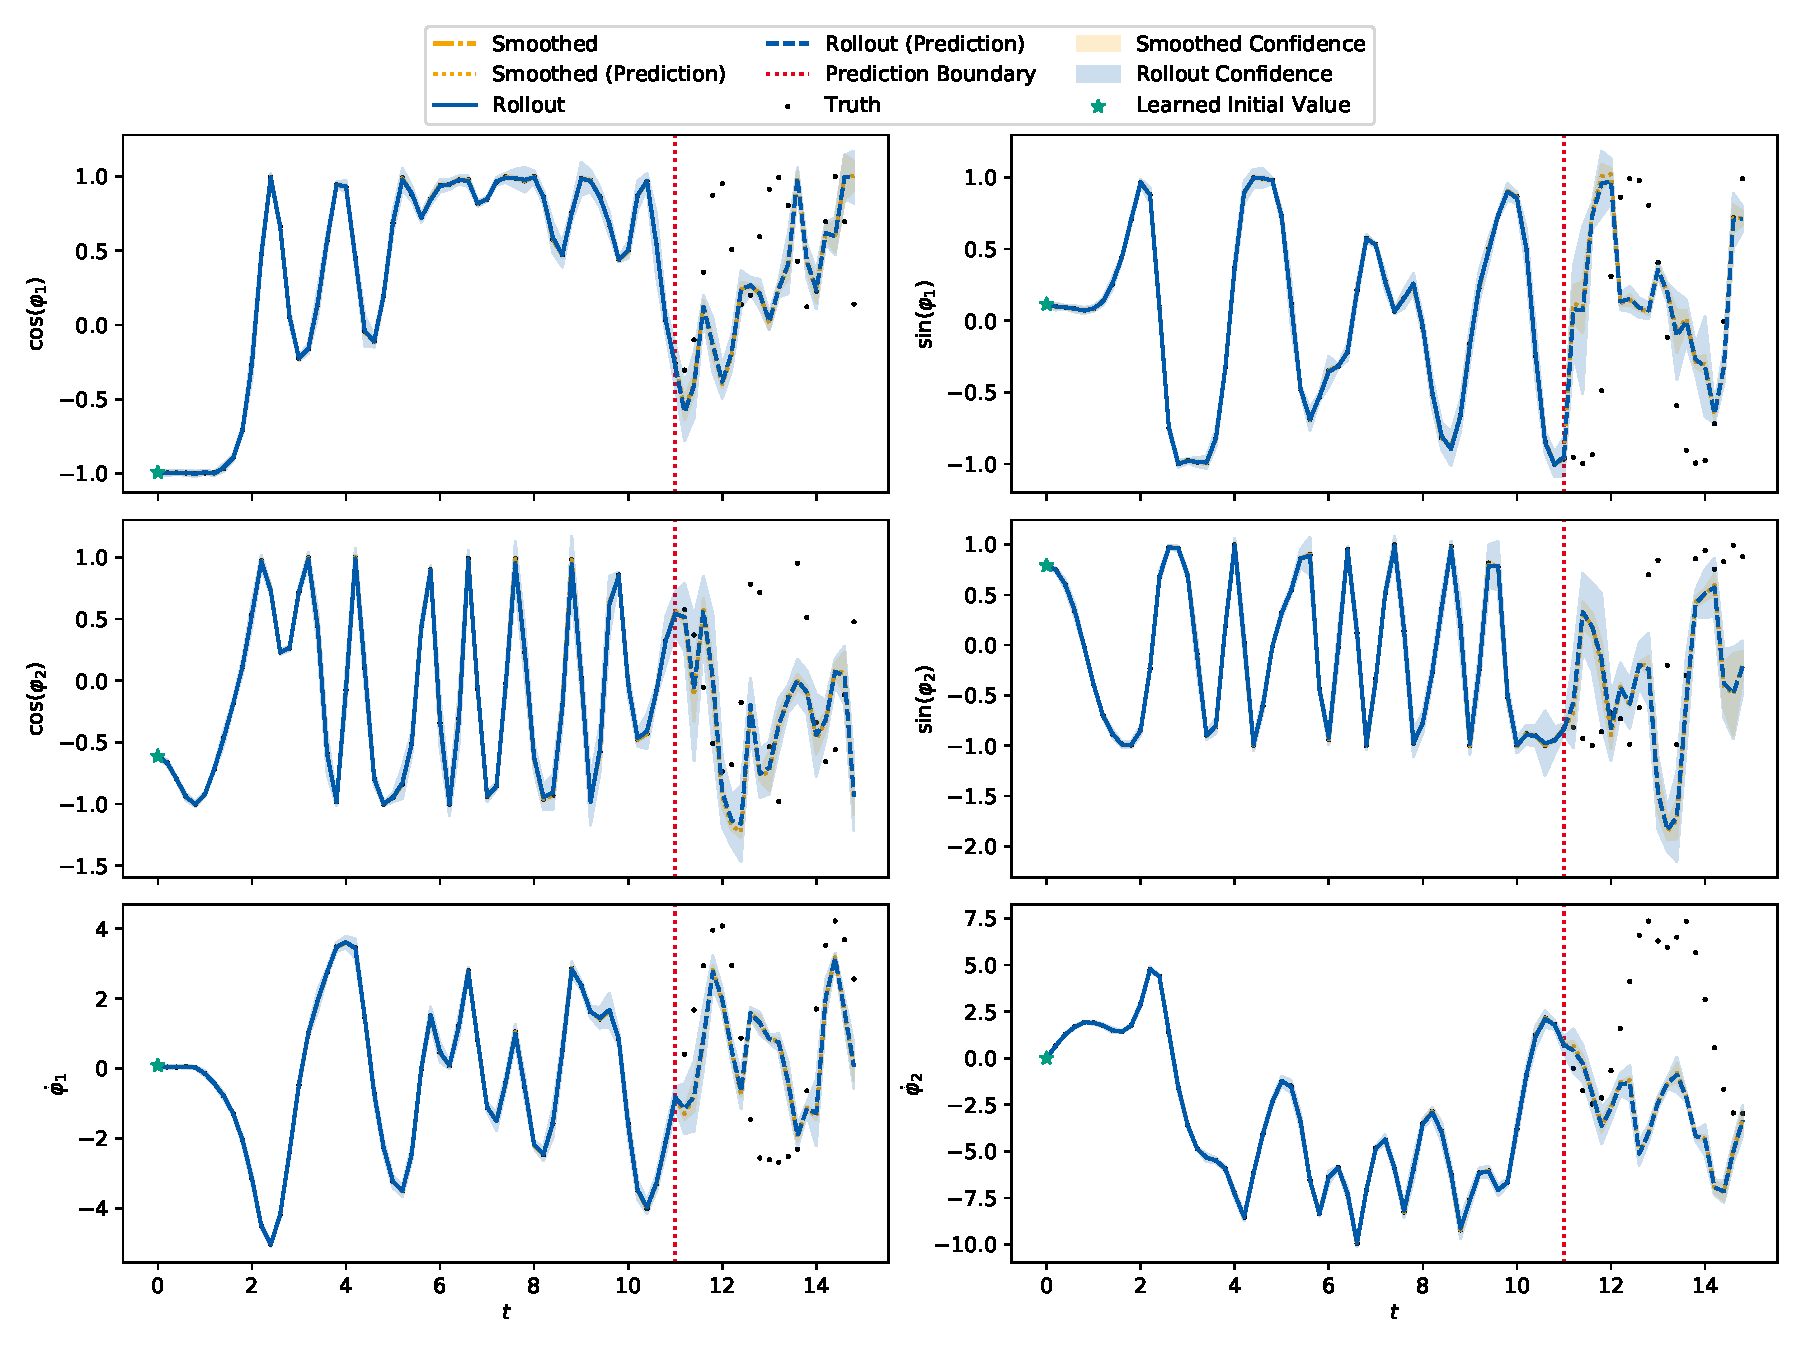
\includegraphics[width=\linewidth]{figures/results/cpu-vs-gpu/acrobot-gpu/rollout-observations-N0.pdf}
			\caption{Rollout of the double pendulum experiment that ran on the \ac{cpu}.}
			\label{fig:cpuVsGpuCpu}
		\end{figure}
		\begin{figure}
			\centering
			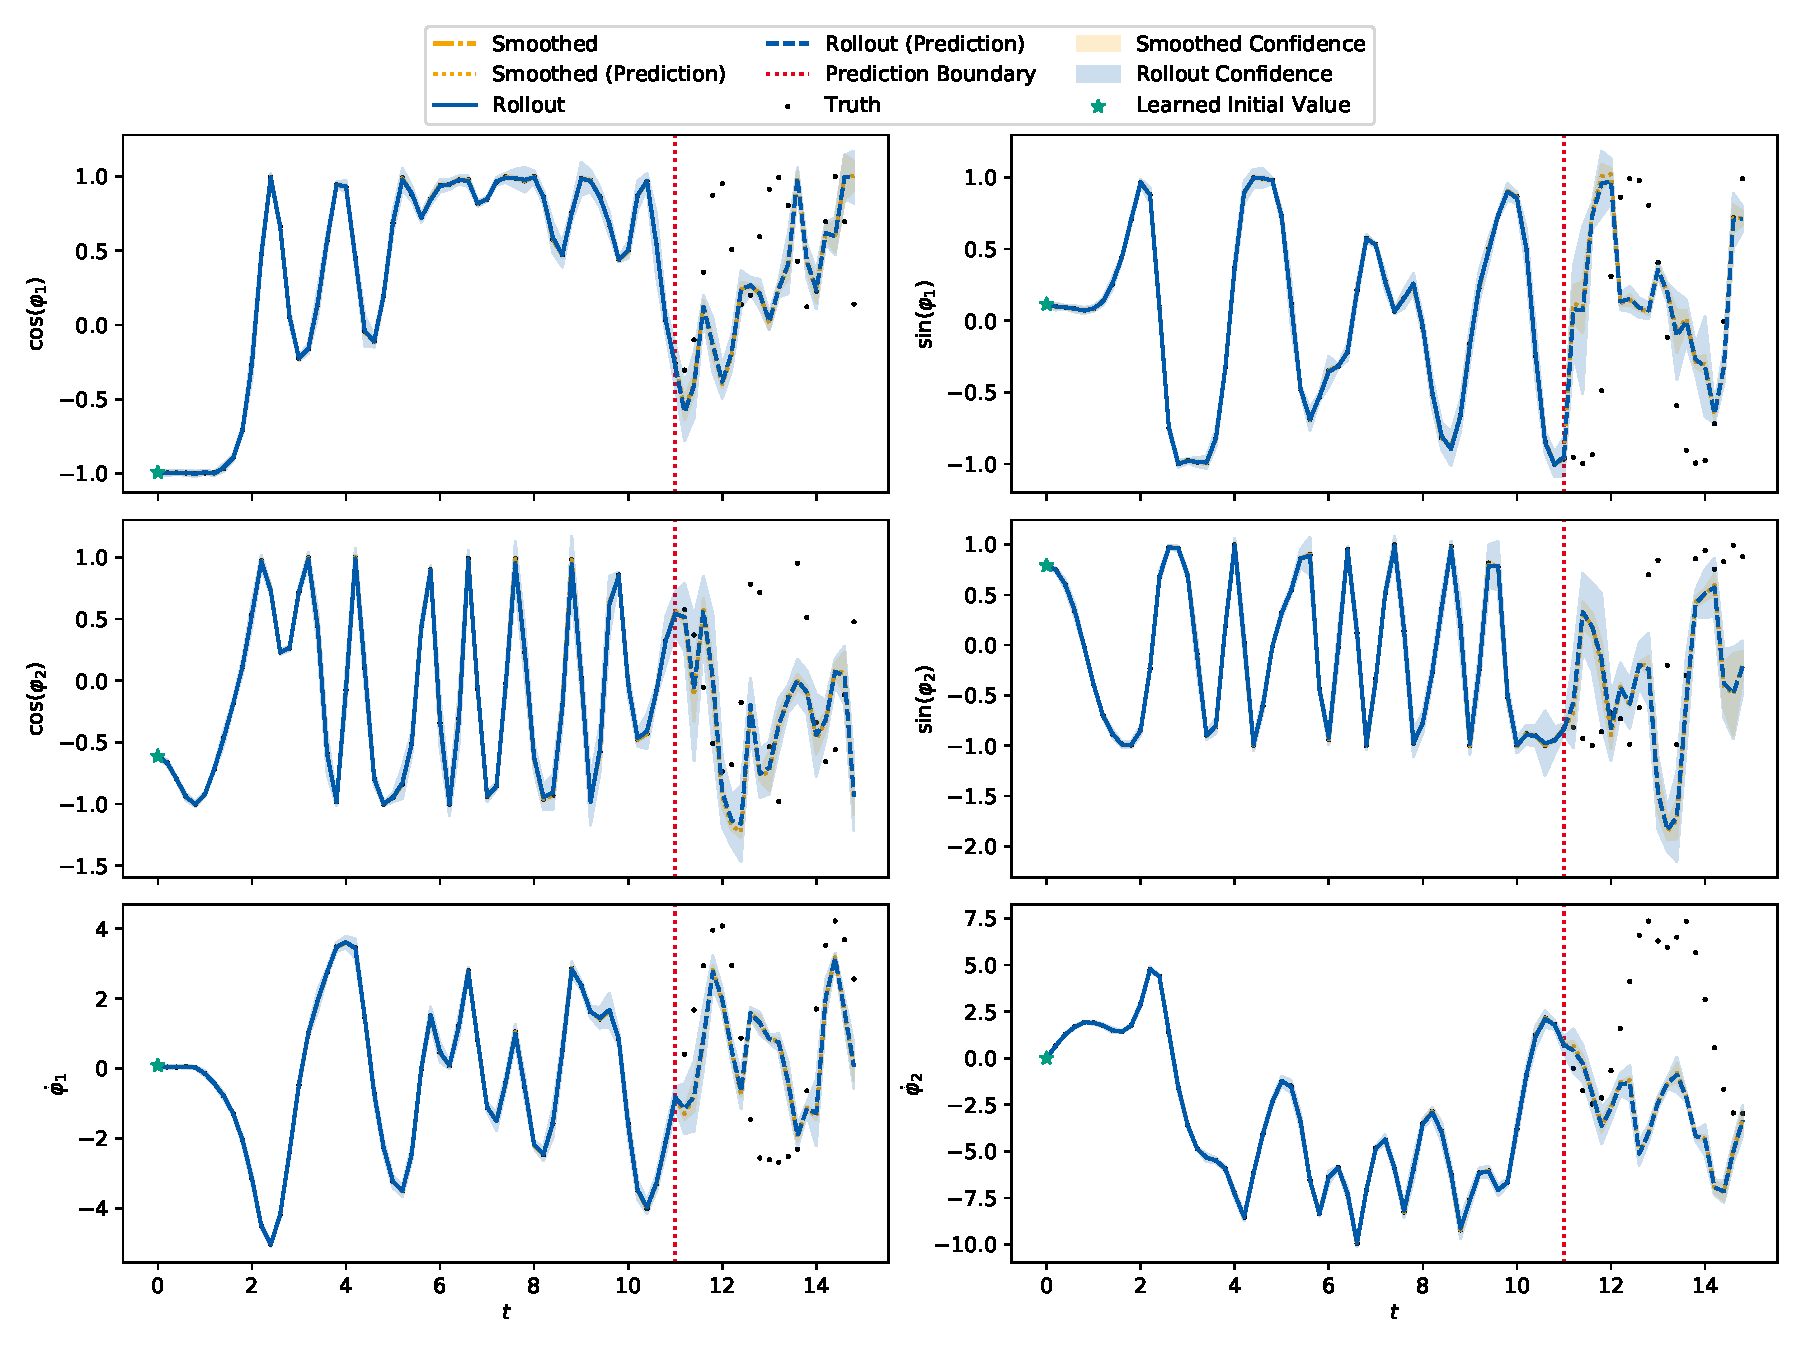
\includegraphics[width=\linewidth]{figures/results/cpu-vs-gpu/acrobot-gpu/rollout-observations-N0.pdf}
			\caption{Rollout of the double pendulum experiment that ran on the \ac{gpu}.}
			\label{fig:cpuVsGpuGpu}
		\end{figure}
	% end
% end
